%%%%%%%%%%%%%%%%%%%%%%%%%%%%%%%%%%%%%%%%%%%%%%%%%%%%%%%%%%%%%%%%%%%%%%%%%%%%%%%%
% IEEE Conference Template - School Bus Routing Project
%%%%%%%%%%%%%%%%%%%%%%%%%%%%%%%%%%%%%%%%%%%%%%%%%%%%%%%%%%%%%%%%%%%%%%%%%%%%%%%%

\documentclass[letterpaper, 10 pt, conference]{ieeeconf}

\IEEEoverridecommandlockouts                             
\overrideIEEEmargins

% --- Packages ---
\usepackage{graphics} 
\usepackage{epsfig} 
\usepackage{amsmath} 
\usepackage{amssymb}  
\usepackage{url}
\usepackage[ruled, vlined, linesnumbered]{algorithm2e}
\usepackage{verbatim} 
\usepackage{soul, color}
\usepackage{lmodern}
\usepackage[utf8]{inputenc}
\usepackage{fourier} 
\usepackage{array}
\usepackage{makecell}
\usepackage{placeins}
\usepackage{booktabs}
\setlength{\textfloatsep}{8pt plus 2pt minus 2pt}
\setlength{\floatsep}{8pt plus 2pt minus 2pt}
\setlength{\intextsep}{8pt plus 2pt minus 2pt}

% --- Hyperref Setup for Clickable Links ---
\usepackage{hyperref}
\hypersetup{
    colorlinks=true,
    linkcolor=black,
    citecolor=black,
    filecolor=blue,      
    urlcolor=blue,
}

\SetNlSty{large}{}{:}

\renewcommand\theadalign{bc}
\renewcommand\theadfont{\bfseries}
\renewcommand\theadgape{\Gape[4pt]}
\renewcommand\cellgape{\Gape[4pt]}

\pagestyle{plain} 

% --- Title and Author ---
\title{\LARGE \bf
Routing Under Passenger Welfare Constraints: Efficiency, Safety, and Comfort in Demand-Responsive Bus Systems — A School Bus Case Study
}

\author{Authors Names\\
Department of Information Technology \\
Misr University For Science And Technology \\
}

\begin{document}

\maketitle
\thispagestyle{plain}
\pagestyle{plain}

%%%%%%%%%%%%%%%%%%%%%%%%%%%%%%%%%%%%%%%%%%%%%%%%%%%%%%%%%%%%%%%%%%%%%%%%%%%%%%%%
\begin{abstract}
This paper presents a demand-responsive optimization framework for the School Bus Routing Problem (SBRP) for developing regions such as Cairo, Egypt, characterized by limited pedestrian infrastructure and informal road usage (jaywalking). We propose a pipeline that balances operator efficiency with passenger welfare and safety. Using real-world OpenStreetMap data, we implement an Adaptive Large Neighborhood Search (ALNS) that integrates safety-aware bus stop generation with school-stage-appropriate walking constraints and proportional ride-time caps. By evaluating the system across a School-Stage-Tiered Safety Framework, ranging from a Direct (Point-to-Point) baseline to Strictly-Constrained and Weakly-Constrained regimes based on school-stage-tiered network permeability, we quantify the ``safety premium'' associated with avoiding potentially hazardous crossings, and the ``comfort premium'' associated with minimal walking and fast rides. Our findings provide a measurable trade-off between fiscal optimization and student well-being, offering a scalable model for schools in developing regions where comprehensive data for public road networks are often scarce.
\end{abstract}

\begin{keywords}
School Bus Routing Problem, Vehicle routing, Stop Selection, Metaheuristic Algorithms
\end{keywords}

%%%%%%%%%%%%%%%%%%%%%%%%%%%%%%%%%%%%%%%%%%%%%%%%%%%%%%%%%%%%%%%%%%%%%%%%%%%%%%%%
\section{INTRODUCTION}

Transportation is a critical yet expensive component of educational infrastructure. In cities like Cairo, the School Bus Routing Problem (SBRP) is further complicated by the scarcity of high-quality, detailed road network data and a lack of formal pedestrian infrastructure, which renders jaywalking the systemic norm. Historically, optimization research has prioritized operator efficiency—minimizing fleet size and total distance—while treating passenger welfare, such as ride-time comfort or pedestrian access, as secondary parameters or static constraints.

This study introduces a pipeline that balances operator efficiency with passenger welfare. We analyze the trade-offs between three core pillars:
\begin{itemize}
    \item \textbf{Efficiency:} The minimization of the active fleet size and total route duration.
    \item \textbf{Safety:} The dynamic selection of bus stops based on student-specific needs and the avoidance of hazardous street crossings.
    \item \textbf{Comfort and Equity:} The enforcement of school-stage-appropriate walking limits and the mitigation of excessive ride times through dynamic, proportional caps. 
\end{itemize}

The core contribution of this work is a School-Stage-Tiered Comparison Framework that isolates the impact of these constraints. By evaluating a Strictly-Constrained safety regime (restricting crossings by school stage and road class) against a Weakly-Constrained model (allowing higher network permeability for older students) and a Direct Point-to-Point baseline, we provide a measurable ``safety premium.'' This research utilizes real-world geospatial data from OpenStreetMap and employs an Adaptive Large Neighbourhood Search (ALNS) to solve the resulting high-dimensional combinatorial problem.

%%%%%%%%%%%%%%%%%%%%%%%%%%%%%%%%%%%%%%%%%%%%%%%%%%%%%%%%%%%%%%%%%%%%%%%%%%%%%%%%
\section{RELATED WORKS}

The SBRP has been extensively studied as a specialized variant of the Vehicle Routing Problem (VRP) \cite{c1}. This section reviews the literature relevant to our three-pillar framework, focusing on stop selection, welfare constraints, and solution approaches for developing world contexts.

\subsection{Problem Decomposition and Classification}
The SBRP is conventionally decomposed into several sub-problems. Desrosiers et al. \cite{c1} established a framework comprising data preparation, bus stop selection, route generation, school bell time adjustment, and route scheduling. A comprehensive review by Wang et al. \cite{c2} confirms that route generation has attracted the predominant share of scholarly attention, while stop selection remains comparatively under-explored, appearing in approximately one-quarter of SBRP publications \cite{c2}.

Our framework follows the location-allocation-routing (LAR) strategy identified by Park and Kim \cite{c1}, where stops are selected and students assigned before routes are generated. Unlike traditional sequential LAR, our framework integrates stop selection within the optimization loop through dynamic candidate generation per student.

\subsection{Stop Selection and Safety Considerations}
The stop selection sub-problem entails assigning students to boarding points while balancing walking distance, safety, and efficiency. Safety in stop selection has received particular attention recently, with guidelines emphasizing the hazards of getting to the stop, such as lack of suitable footpaths or crossing points. Despite these advances, literature often assumes stop locations as fixed inputs \cite{c3}. Our work extends this by generating candidate stops dynamically via safety-filtered BFS.

\subsection{Passenger Welfare: Scaling Service Quality to Geographic Reality}
Traditional SBRP models typically enforce service quality through a static, uniform maximum ride time ($T_{max}$). However, a fixed cap is fundamentally ``geographically blind,'' as it fails to account for the spatial diversity of a school’s catchment area. In a large-scale urban network, a single value for $T_{max}$ (e.g., 60 minutes) forces a rigid, binary threshold for all students regardless of their proximity. 



To address this, we propose a \textit{Dynamic Proportional Cap} (formulated in Section III-B) which scales the allowable ride time to the student's direct distance, ensuring equity between short and long commutes.

\subsection{Metaheuristic Solution Approaches}
Given the NP-hard nature of SBRP \cite{c2}, metaheuristics dominate the landscape. Adaptive Large Neighbourhood Search (ALNS) has emerged as an effective approach for complex SBRP sub-classes. Its success is due to the adaptive selection of operators \cite{c7}, which allow the algorithm to target specific constraint violations through various destroy-and-repair mechanisms.

\subsection{Developing World Applications and Research Gaps}
Cairo's road environment is characterized by limited pedestrian infrastructure and informal crossing behavior, directly motivating our safety-constrained mode. Developed-world assumptions regarding pedestrian safety and bus stop access cannot be transferred uncritically to such contexts. Our work addresses several identified research gaps:
\begin{itemize}
    \item \textbf{Safety-Aware Stop Generation via School-Stage-Tiered Permeability:} Unlike traditional models that treat the road network as a uniform graph, our approach integrates pedestrian route safety into the candidate stop generation phase via a school-stage safety matrix. This filters the network based on a student’s school stage, ensuring Tertiary and Secondary roads are treated as impassable barriers for younger students while permitting ``Weakly-Constrained'' access for older age groups.
    \item \textbf{Dynamic Welfare Constraints:} Existing formulations predominantly employ static ride-time maximums \cite{c1, c5}. A dynamic cap proportional to $T_{direct}$ provides a more equitable service level.
    \item \textbf{The School-Stage-Tiered Comparison Framework:} Quantifying the marginal costs of welfare constraints by comparing regimes (Strictly-Constrained, Weakly-Constrained, and Direct) with varying levels of network access and student-walking requirements.
\end{itemize}

\begin{table}[h]
\centering
\caption{\textbf{Summary of Related Work Positioning}}
\label{tab:positioning}
\begin{tabular}{|>{\raggedright\arraybackslash}p{0.2\linewidth}|>{\raggedright\arraybackslash}p{0.25\linewidth}|>{\raggedright\arraybackslash}p{0.4\linewidth}|}
\hline
\textbf{Theme} & \textbf{Representative Study} & \textbf{Our Extension} \\
\hline
Stop Selection & \cite{c1, c3} & Safety-filtered BFS candidate generation \\
\hline
Safety & \cite{c1, c2} & Road classification as safe\_to\_cross \\
\hline
Ride Time & \cite{c1, c5} & Dynamic proportional caps ($k \times T_{direct}$) \\
\hline
Methodology & \cite{c7} & Adaptive destroy-repair ALNS with welfare-aware feasibility checks \\
\hline
Context & \cite{c5} & Cairo OSMnx implementation \\
\hline
\end{tabular}
\end{table}

%%%%%%%%%%%%%%%%%%%%%%%%%%%%%%%%%%%%%%%%%%%%%%%%%%%%%%%%%%%%%%%%%%%%%%%%%%%%%%%%
\section{PROBLEM DESCRIPTION AND FORMULATION}

The \textit{Welfare-Aware School Bus Routing Problem (WA-SBRP)} is solved on a directed road graph $G=(V,A)$ built from OpenStreetMap travel-time edges. Let $S$ be students, $R$ be bus routes, and $P$ be candidate pickup nodes generated from student-centered pedestrian reachability. In the implemented model, each route is school-anchored (pickup sequence ending at the school node) and students may remain unserved when no feasible insertion exists. Therefore, the optimization is a constrained \textit{service maximization} model, not a strict all-served minimization model.

\subsection{The Objective Function}
We maximize a weighted score that prioritizes serving students, then compact routing, while penalizing long bus travel and excessive walking:

\begin{equation}
\max F = w_s\!\sum_{s\in S} y_s - w_r\!\sum_{r\in R} z_r - \sum_{r\in R} T_r - \sum_{s\in S} \phi_s
\end{equation}

where $y_s\in\{0,1\}$ indicates whether student $s$ is served, $z_r\in\{0,1\}$ indicates whether route $r$ is active, $T_r$ is route travel time, and $\phi_s$ is the walking penalty for student $s$. The implementation uses $w_s=10000$ and $w_r=5000$, which ensures one additional served student dominates the activation of one additional bus.

\subsection{Passenger Welfare Constraints}
The WA-SBRP transforms welfare into geographic and temporal constraints with a hard-feasibility layer (candidate generation and insertion checks) and a soft-cost layer (walking penalty in the objective):

\begin{enumerate}
    \item \textbf{School-Stage-Tiered Network Permeability (Safety):} For each student $s$, the pedestrian exploration graph is filtered by road safety permissions defined for their school stage.
    \item \textbf{School-Stage Walking Eligibility:} A stop $p$ is a feasible candidate for student $s$ only if pedestrian distance in the filtered graph satisfies $d_{walk}(s,p)\le W_{stage(s)}$.
    \item \textbf{Dynamic Proportional Ride-Time Cap:} To prevent specific geographical discrimination, we define a feasibility corridor for the maximum ride time $T^{\max}_s$:
    \begin{equation}
    T^{\max}_s = \max\left(\tau_{\mathrm{min}},\min\left(k\,T^{direct}_s,\;T^{direct}_s+\tau_{\mathrm{add}}\right)\right)
    \end{equation}
    
This logic establishes a ``feasibility corridor'' serving three objectives:
\begin{enumerate}
    \item \textbf{The Floor (Operational Efficiency):} Sets a minimum baseline enrolling students can expect (e.g., 45 min) to ensure the system remains efficient without constraining the optimization too much by students who live really close to the school (eg. 10 min away).
    \item \textbf{The Multiplier ($k$):} Maintains a consistent service quality ratio for the median student population.
    \item \textbf{The Additive Ceiling (Student Comfort):} Imposes an absolute cap especially relevant for long-distance commutes where the multiplicative nature of  $k\,T^{direct}_s$ leads to an unacceptable $T^{\max}_s$ for students who live far away.
\end{enumerate}
    \item \textbf{Configurable Directional Enforcement:} Let $T^{AM}_s$ and $T^{PM}_s$ denote morning and afternoon in-vehicle times. In strict directional mode, insertion requires $T^{AM}_s\le T^{\max}_s$. In bidirectional-lenient mode (default), insertion is rejected only when both directions violate the cap:
    \begin{equation}
    \text{reject iff } \left(T^{AM}_s>T^{\max}_s\right) \wedge \left(T^{PM}_s>T^{\max}_s\right)
    \end{equation}
    \item \textbf{Walking Penalty Layer:} Even among feasible candidates, longer walks are penalized in the objective by $\phi_s$; non-computable walking paths receive a heavy fallback penalty, discouraging but not hard-forbidding assignment.
\end{enumerate}

\subsection{Operational Constraints}
\begin{itemize}
    \item \textbf{Capacity:} For each route $r$, assigned students satisfy $\sum_{s\in S_r}1 \le Q_r$.
    \item \textbf{School-Anchored Route Structure:} Each route is an ordered pickup sequence terminating at the school node.
    \item \textbf{Single Assignment for Served Students:} Each served student is assigned to exactly one stop on one route. Unserved students are allowed and reflected through reduced objective value.
    \item \textbf{Insertion Feasibility:} Candidate insertions must satisfy capacity and ride-time rules for both the inserted student and previously assigned downstream students.
\end{itemize}

%%%%%%%%%%%%%%%%%%%%%%%%%%%%%%%%%%%%%%%%%%%%%%%%%%%%%%%%%%%%%%%%%%%%%%%%%%%%%%%%
\section{PROPOSED METHOD}

This section details the computational framework developed to solve the Welfare-Aware School Bus Routing Problem (WA-SBRP). The approach integrates geospatial data processing, dynamic candidate stop generation based on pedestrian safety heuristics, and a tailored metaheuristic optimizer. We first outline the end-to-end pipeline before detailing the synthetic data generation, network augmentation strategies, and the core routing algorithm.

\subsection{Pipeline Overview}
The implemented workflow follows five stages:
\begin{enumerate}
    \item \textbf{Data Generation and Graph Construction:} Synthesize student populations via an annulus-based distribution around the school (Algorithm~\ref{alg:synthetic_data_gen}), build drive and pedestrian graphs from OpenStreetMap, and cache reusable artifacts.
    \item \textbf{School-Stage-Tiered Candidate Generation:} For each student, perform safety-filtered pedestrian search to enumerate reachable pickup nodes under mode-specific crossing rules (Strictly-Constrained, Weakly-Constrained, or Direct).
    \item \textbf{Pedestrian Graph Augmentation:} Inject synthetic pedestrian crossings between opposite carriageways (when safety predicates hold) to model informal crossing behavior not represented in car-centric topology.
    \item \textbf{ALNS Route Optimization:} Solve the service-maximization objective with destroy-repair neighborhoods and simulated-annealing acceptance.
    \item \textbf{Experiment Logging and Comparison:} Export per-mode outputs including objective progression, operator statistics, crossing metrics, and timing telemetry.
\end{enumerate}

\subsection{Synthetic Dataset Generation}
Due to privacy constraints and the lack of publicly available school registries in the studied region, student home locations are synthetically generated using a Gaussian annulus-based spatial distribution model. Rather than distributing students uniformly across the map, this approach more accurately models real-world school catchments where the density of bus-riding students is highest in a "commuter ring" at a specific distance from the school.

Centered on a selected real-world school node, the generation process samples a student's distance from the school using a bounded Gaussian distribution (e.g., concentrated around a peak distance of 2.0 km with a specified standard deviation). To prevent unrealistic edge cases, generated distances that fall outside predefined minimum (e.g., 0.4 km) and maximum bounds are discarded and resampled. Then a uniformly random angle ($0$ to $2\pi$) is selected to determine the direction bearing. Finally, these polar variables (distance and angle) are translated into geographical latitude and longitude coordinates. Algorithm~\ref{alg:synthetic_data_gen} summarizes the exact generation workflow used for experiments.

Each generated student is assigned a specific school stage based on the school's specific demographics; otherwise we assume a uniform distribution of students across all school stages, which subsequently governs their allowable walking limits and safety-filtered permissions for crossing roads.

\begin{algorithm}[!t]
\caption{Synthetic Student Dataset Generation (Annulus-Gaussian)}
\label{alg:synthetic_data_gen}
\KwIn{School center $(\phi_c,\lambda_c)$, number of students $N$, distance bounds $[d_{min}, d_{max}]$, Gaussian parameters $(\mu_d,\sigma_d)$, stage policy}
\KwOut{Student set $S$ with coordinates and school stages}
$S \leftarrow \emptyset$\;
\For{$i \leftarrow 1$ \KwTo $N$}{
    Sample $d \sim \mathcal{N}(\mu_d,\sigma_d)$ until $d_{min} \le d \le d_{max}$\;
    Sample $\theta \sim \mathcal{U}(0, 2\pi)$\;
    Convert polar offset $(d,\theta)$ around $(\phi_c,\lambda_c)$ to geographic point $(\phi_i,\lambda_i)$\;
    Sample school stage $g_i$ from configured stage distribution (or uniform fallback)\;
    Create student $s_i=(\phi_i,\lambda_i,g_i)$ and append to $S$\;
}
\Return{$S$}\;
\end{algorithm}

\subsection{Candidate Stop Generation and Safety Modes}
Candidate stops are not predefined; they are generated dynamically from each student location using pedestrian reachability under road-class safety rules. The three comparison modes are:
\begin{itemize}
    \item \textbf{Strictly-Constrained:} conservative crossing permissions by school stage.
    \item \textbf{Weakly-Constrained:} increased permeability, especially for older stages.
    \item \textbf{Direct (Point-to-Point):} walking suppressed (effectively home pickup), used as a baseline.
\end{itemize}

\subsection{Pedestrian Graph Augmentation via Synthetic Crossings}
OpenStreetMap drive topology frequently represents divided roads as two opposite carriageways without direct pedestrian edge between sides. In Egypt-like contexts, this causes us to not be able to model crossing streets (jaywalking) if the candidate generation relies only on the native car-network. To address this, we augment the \emph{pedestrian} graph with synthetic crossing edges between opposite sides of eligible roads (typically tertiary/secondary classes) when geometric and safety checks are satisfied. These synthetic edges are used only for pedestrian reachability and stop-candidate generation; bus routing remains on the original directed drive graph. This separation preserves vehicular realism while enabling context-faithful modeling of informal crossing behavior.

Algorithm~\ref{alg:candidate_synth} summarizes the integrated stop-candidate pipeline. It combines school-stage safety permissions with synthetic crossing augmentation before bounded pedestrian exploration and ranking to generate the feasible insertion universe. The dominant runtime comes from bounded graph traversal on the augmented walk graph; with neighborhood-bounded search, practical behavior is near-linear in explored edges per student. This step is critical because it decides the feasible insertion universe seen by the ALNS optimizer.

\begin{algorithm}[h]
\caption{Safety-Aware Candidate Generation with Synthetic Crossings}
\label{alg:candidate_synth}
\KwIn{Drive graph $G_d$, pedestrian graph $G_w$, student $s$, school-stage policy $\Pi$, mode config}
\KwOut{Ranked candidate stop set $C_s$}
Construct stage-filtered pedestrian permissions for $s$ from $\Pi$\;
Detect eligible opposite-carriageway pairs under geometry and road-class rules\;
Insert synthetic crossing edges into $G_w$ only when safety predicates are satisfied\;
Run bounded pedestrian search from student frontage/home node on augmented $G_w$\;
Map reachable pedestrian nodes to drive-graph stop nodes\;
Score and rank candidates (safety, walk distance, consolidation potential)\;
Truncate to top-$K$ mode-dependent candidates\;
\Return{$C_s$}\;
\end{algorithm}

\subsection{ALNS Design}
The optimizer uses an Adaptive Large Neighbourhood Search (ALNS) to solve the service-maximization objective. ALNS employs roulette-wheel operator selection with adaptive weight updates, allowing the algorithm to dynamically choose the most effective destroy and repair strategies based on recent success. Destroy operators include random removal, worst-cost removal, relatedness (Shaw-style) removal, sequence removal, and route-merge removal. Repair uses regret-based insertion as the primary reconstruction policy, with random-order best insertion as a diversification companion. Acceptance follows a simulated annealing (SA) criterion. Stopping is hybrid: no-improvement patience, freeze-based stopping when temperature becomes very low, and wall-clock budget termination (after a minimum-iteration floor). To eliminate excessive computation when an optimal state is reached, the optimizer employs a \textit{satisficing polishing window}: if all students are served and the active fleet size matches the theoretical minimum ($\lceil |S| / C \rceil$), the patience window is tightened to a small constant (30 iterations). After the main loop, if all students are served but active fleet exceeds the theoretical minimum, an optional short merge-focused tail (route-merge destroy + regret repair) attempts additional fleet consolidation. A final repair pass then attempts to insert any remaining unserved students.

\begin{algorithm}[!t]
\caption{ALNS Framework Loop}
\label{alg:alns_loop}
\KwIn{Initial solution $x_0$, destroy set $\mathcal{D}$, repair set $\mathcal{R}$, temperature $T_0$, cooling $\gamma$, patience limit $P_{max}$, time budget $B$, iteration floor $I_{floor}$, freeze threshold $T_{freeze}$, freeze patience $P_{freeze}$, merge-tail iterations $M$}
\KwOut{Best solution $x^*$}
$x \leftarrow x_0$; $x^* \leftarrow x_0$; initialize operator weights and scores\;
$P_{current} \leftarrow P_{max}$ ; $stagnation \leftarrow 0$\;
\For{$it \leftarrow 1$ \KwTo $it_{max}$}{
    \If{$it > I_{floor}$ and elapsed wall-clock $\ge B$}{
        \textbf{break} \tcp*{Time budget stop}
    }
    Select destroy $d \in \mathcal{D}$ and repair $r \in \mathcal{R}$ via roulette-wheel over adaptive weights\;
    $x' \leftarrow r(d(x))$\;
    \If{$f(x') > f(x)$}{
        $x \leftarrow x'$\;
    }
    \Else{
        Accept $x'$ with SA probability $\exp((f(x')-f(x))/T)$\;
    }
    Update operator scores and weights from solution quality signal\;
    \If{$f(x) > f(x^*)$}{
        $x^* \leftarrow x$\;
        $stagnation \leftarrow 0$\;
    }
    \Else{
        $stagnation \leftarrow stagnation + 1$\;
    }
    \If{all served in $x^*$ and active buses $\le \lceil |S|/C \rceil$}{
        $P_{current} \leftarrow \min(P_{current}, 30)$ \tcp*{Polishing window}
    }
    \If{$it \ge I_{floor}$ and $stagnation \ge P_{current}$}{
        \textbf{break} \tcp*{Early stop triggered}
    }
    \If{$it \ge I_{floor}$ and $T \le T_{freeze}$ and $stagnation \ge P_{freeze}$}{
        \textbf{break} \tcp*{Frozen search stop}
    }
    $T \leftarrow \gamma T$\;
}
\If{merge-tail enabled and all served and active buses $> \lceil |S|/C \rceil$}{
    run $M$ merge-focused iterations under remaining budget\;
}
run one final repair pass for any unserved students\;
\Return{$x^*$}\;
\end{algorithm}

Algorithm~\ref{alg:alns_loop} presents the implemented outer search structure, including time-budget and freeze-aware stopping, the satisficing polishing window, and the post-loop consolidation/rescue phases. Each main ALNS iteration costs one destroy, one repair, and one acceptance decision; empirical runtime is dominated by insertion feasibility checks inside repair.

\subsection{Constraint Handling in Search}
Each insertion is validated through a feasibility routine that checks bus capacity and personalized ride-time caps. The ride-time check supports two policies: morning-only strict enforcement or bidirectional leniency (default), where an insertion is rejected only if both AM and PM exceed the personalized cap. This design preserves welfare protection while reducing over-rejection caused by directional asymmetry in one-way street networks.

Algorithm~\ref{alg:insertion_eval} gives the detailed feasibility evaluator used by repair operators. This evaluator is the main source of computational load during repair, because each candidate may trigger AM/PM cap checks plus downstream consistency checks for already assigned students. The benefit is strict welfare-feasibility control without requiring post-hoc repair of invalid routes.

\begin{algorithm}[!t]
\caption{Feasibility-Aware Insertion Evaluation}
\label{alg:insertion_eval}
\KwIn{Route $r$, student $s$, candidate stop $p$, insertion index $i$, cache/matrix, cap parameters}
\KwOut{Valid insertion flag and penalized insertion cost}
Compute detour delta cost for inserting $p$ at index $i$\;
\If{capacity would be violated}{reject}\;
Compute AM ride for $s$ after insertion and personalized cap $T_s^{\max}$\;
\If{strict directional mode and $T_s^{AM} > T_s^{\max}$}{reject}\;
\If{bidirectional-lenient mode and $T_s^{AM} > T_s^{\max}$}{
    compute $T_s^{PM}$ on reversed PM sequence\;
    \If{$T_s^{PM} > T_s^{\max}$}{reject}\;
}
Re-check impacted existing students for post-insertion cap violations\;
Compute walking penalty $\phi_s$ for $s \rightarrow p$\;
\If{walking is infeasible}{reject}\;
\Return{valid, $(\text{detour delta} + \phi_s)$}\;
\end{algorithm}

\FloatBarrier

%%%%%%%%%%%%%%%%%%%%%%%%%%%%%%%%%%%%%%%%%%%%%%%%%%%%%%%%%%%%%%%%%%%%%%%%%%%%%%%%
\section{EXPERIMENTS}

\subsection{Experimental Design}
Mode A is \emph{Strictly-Constrained}, Mode B is \emph{Weakly-Constrained}, and
Mode C is \emph{Direct (Door-to-Door)}. This section defines hypotheses,
environment, datasets, and evaluation protocol before presenting results.

\subsubsection{Research Hypotheses}
\textbf{H1 (Efficiency):} Allowing limited walking (Mode B) improves operational
efficiency relative to both strict safety (Mode A) and door-to-door (Mode C).
\textbf{Primary metrics:} active routes (buses used), total route time (min),
total route distance (km), and average occupancy
$\left(\text{students served} / \text{routes}\right)$.

\textbf{H2 (Safety):} Strict safety constraints (Mode A) reduce walking exposure
without permitting unsafe crossings.
\textbf{Primary metrics:} walking distance statistics (mean, median, max) and
walk utilization rate. Unsafe crossing counts are expected to be zero by
design, because synthetic crossings are not generated on dangerous road
classes; thus safety is interpreted through reduced walking exposure and
compliance with stage-specific limits.

\textbf{H3 (Comfort):} Door-to-door service (Mode C) minimizes walking but can
increase ride burden and efficiency cost; comfort gains are not free.
\textbf{Primary metrics:} walking distance statistics, ride-cap violation counts
and rates, and per-student travel burden
$\left(\text{total route time} / \text{students served}\right)$.

\textbf{H4 (Scalability / Search-Space Bottleneck):} At larger scales,
candidate-space size dominates solver throughput, so smaller candidate sets
(Mode C) yield higher iterations per second and faster convergence under fixed
time budgets, even if they are not operationally optimal in smaller instances.
\textbf{Primary metrics:} executed iterations, iterations per second, candidate
counts considered, and served counts at large $|S|$. We anchor the scalability
claim at $|S|=400$ (fully matched cohorts).

\subsubsection{Simulation Environment and Hardware}
All modes are executed in the same software pipeline and under identical
algorithmic settings per paired seed. To support reproducibility and IEEE-style
reporting, this subsection should include the exact execution stack used for
the final runs:
\begin{itemize}
    \item CPU model and core/thread count.
    \item RAM capacity.
    \item Operating system and version.
    \item Python version and key package versions.
\end{itemize}
\subsubsection{Dataset Description}
We evaluated the three modes on synthetic datasets generated around a fixed
school location, using the annulus distribution described in Section IV-B. We
used Victory College School (Maadi, Cairo) as the anchor site and a bounded
study area around Maadi to keep computation tractable. The bounding box corners
were $(29.991682,31.331909)$ and $(29.92563,31.229084)$, corresponding to
approximately $72.76\,\text{km}^2$. Students were generated only inside this
bounding box.
Each instance size uses multiple random seeds to capture geographic
variability. For each seed, all three modes are run on the same student set,
ensuring paired comparison across modes. Unless otherwise stated, algorithm
parameters (time budget, candidate cap, destroy/repair operators, and
ride-time constraints) are held constant across modes.

\subsubsection{Evaluation Metrics}
We report solution quality using four groups of metrics:
\begin{itemize}
    \item \textbf{Coverage:} students served, students unserved, and served rate.
    \item \textbf{Efficiency:} active routes (buses used), total route time,
    total route distance, and average occupancy
    $\left(\text{students served} / \text{routes}\right)$.
    \item \textbf{Comfort:} walking distance statistics (mean/median/max), walk
    utilization rate, and ride-cap violation counts or rates.
    \item \textbf{Runtime and Scalability:} executed iterations, iterations per
    second, and candidate breadth proxies (e.g., candidates considered or
    critical matrix nodes).
\end{itemize}

\subsubsection{Paired Comparison Protocol}
For each instance size, we compute per-seed differences between modes
(e.g., Mode A minus Mode B) and test whether the median paired difference is
significantly different from zero using the Wilcoxon signed-rank test. This
controls for seed-specific geography, so differences are attributed to the mode
rather than random layout effects. We report mean $\pm$ SD descriptively,
Wilcoxon $p$-values inferentially, and rank-biserial correlation as effect
size. Across each hypothesis-family of comparisons, $p$-values are adjusted via
Holm-Bonferroni ($\alpha=0.05$). Formal inference uses complete matched cohorts
($|S|\in\{100,200,400\}$).

\input{tables/table1_aggregate_metrics.tex}

\begin{table*}[!t]
\centering
\caption{Wilcoxon Paired Comparisons with Holm-Corrected p-values and Rank-Biserial Effect Size}
\label{tab:wilcoxon_effects}
\scriptsize
\setlength{\tabcolsep}{3pt}
\resizebox{\textwidth}{!}{%
\begin{tabular}{rllrrrrrrrr}
\toprule
cohort & comparison & metric & n pairs & median delta & mean delta & wilcoxon W & p raw & effect rank biserial & p holm & significant alpha 0 05 \\
\midrule
100 & Mode A - Mode B & alns\_runtime\_seconds & 5 & -5.450000 & -11.424000 & 1.000000 & 0.125000 & -0.866667 & 1.000000 & False \\
100 & Mode A - Mode B & routes\_created & 5 & 1.000000 & 0.800000 & 0.000000 & 0.125000 & 1.000000 & 1.000000 & False \\
100 & Mode A - Mode B & served\_rate\_pct & 5 & 1.000000 & 0.400000 & 3.500000 & 0.750000 & 0.300000 & 1.000000 & False \\
100 & Mode A - Mode B & total\_route\_dist\_km & 5 & 13.940000 & 12.832000 & 1.000000 & 0.125000 & 0.866667 & 1.000000 & False \\
100 & Mode A - Mode B & total\_route\_time\_min & 5 & 36.160000 & 34.150000 & 0.000000 & 0.062500 & 1.000000 & 1.000000 & False \\
100 & Mode B - Mode C & alns\_runtime\_seconds & 5 & 31.930000 & 33.106000 & 0.000000 & 0.062500 & 1.000000 & 1.000000 & False \\
100 & Mode B - Mode C & avg\_walk\_dist\_m & 3 & 81.900000 & 87.500000 & 0.000000 & 0.250000 & 1.000000 & 1.000000 & False \\
100 & Mode B - Mode C & routes\_created & 5 & -1.000000 & -0.800000 & 0.000000 & 0.125000 & -1.000000 & 1.000000 & False \\
100 & Mode B - Mode C & served\_rate\_pct & 5 & 2.000000 & 2.200000 & 0.000000 & 0.125000 & 1.000000 & 1.000000 & False \\
100 & Mode B - Mode C & total\_route\_dist\_km & 5 & -12.500000 & -14.794000 & 1.000000 & 0.125000 & -0.866667 & 1.000000 & False \\
100 & Mode B - Mode C & total\_route\_time\_min & 5 & -43.780000 & -43.522000 & 0.000000 & 0.062500 & -1.000000 & 1.000000 & False \\
200 & Mode A - Mode B & alns\_runtime\_seconds & 5 & -21.000000 & -18.856000 & 0.000000 & 0.125000 & -1.000000 & 1.000000 & False \\
200 & Mode A - Mode B & routes\_created & 5 & 1.000000 & 0.800000 & 0.000000 & 0.125000 & 1.000000 & 1.000000 & False \\
200 & Mode A - Mode B & served\_rate\_pct & 5 & 2.000000 & 1.600000 & 1.500000 & 0.187500 & 0.800000 & 1.000000 & False \\
200 & Mode A - Mode B & total\_route\_dist\_km & 5 & 23.490000 & 22.926000 & 0.000000 & 0.062500 & 1.000000 & 1.000000 & False \\
200 & Mode A - Mode B & total\_route\_time\_min & 5 & 56.850000 & 61.190000 & 0.000000 & 0.062500 & 1.000000 & 1.000000 & False \\
200 & Mode B - Mode C & alns\_runtime\_seconds & 5 & 21.000000 & 35.170000 & 0.000000 & 0.062500 & 1.000000 & 1.000000 & False \\
200 & Mode B - Mode C & routes\_created & 5 & -1.000000 & -1.200000 & 0.000000 & 0.062500 & -1.000000 & 1.000000 & False \\
200 & Mode B - Mode C & served\_rate\_pct & 5 & -2.500000 & -2.300000 & 0.000000 & 0.125000 & -1.000000 & 1.000000 & False \\
200 & Mode B - Mode C & total\_route\_dist\_km & 5 & -40.720000 & -37.026000 & 0.000000 & 0.062500 & -1.000000 & 1.000000 & False \\
200 & Mode B - Mode C & total\_route\_time\_min & 5 & -104.110000 & -100.066000 & 0.000000 & 0.062500 & -1.000000 & 1.000000 & False \\
400 & Mode A - Mode B & alns\_runtime\_seconds & 5 & -0.010000 & -14.538000 & 2.000000 & 0.250000 & -0.733333 & 1.000000 & False \\
400 & Mode A - Mode B & routes\_created & 5 & 1.000000 & 0.600000 & 0.000000 & 0.250000 & 1.000000 & 1.000000 & False \\
400 & Mode A - Mode B & served\_rate\_pct & 5 & 3.500000 & 3.150000 & 0.000000 & 0.062500 & 1.000000 & 1.000000 & False \\
400 & Mode A - Mode B & total\_route\_dist\_km & 5 & 18.080000 & 19.260000 & 3.000000 & 0.312500 & 0.600000 & 1.000000 & False \\
400 & Mode A - Mode B & total\_route\_time\_min & 5 & 94.330000 & 93.042000 & 0.000000 & 0.062500 & 1.000000 & 1.000000 & False \\
400 & Mode B - Mode C & alns\_runtime\_seconds & 5 & 9.010000 & 47.170000 & 0.000000 & 0.062500 & 1.000000 & 1.000000 & False \\
400 & Mode B - Mode C & routes\_created & 5 & -1.000000 & -1.000000 & 0.000000 & 0.062500 & -1.000000 & 1.000000 & False \\
400 & Mode B - Mode C & served\_rate\_pct & 5 & -4.250000 & -4.100000 & 0.000000 & 0.062500 & -1.000000 & 1.000000 & False \\
400 & Mode B - Mode C & total\_route\_dist\_km & 5 & -51.840000 & -45.094000 & 1.000000 & 0.125000 & -0.866667 & 1.000000 & False \\
400 & Mode B - Mode C & total\_route\_time\_min & 5 & -150.190000 & -154.586000 & 0.000000 & 0.062500 & -1.000000 & 1.000000 & False \\
\bottomrule
\end{tabular}

}
\end{table*}


\section{RESULTS AND DISCUSSION}
This section reports the empirical outcomes and interprets them with
respect to H1--H4.

\subsubsection{Comparative Analysis}
Aggregate results (Table~\ref{tab:aggregate_metrics}) show a stable operational
trade-off across complete cohorts. Mode B consistently reduced route-time and
route-distance relative to Mode A (e.g., at $|S|=400$, $711.22\pm62.31$ min vs
$804.26\pm29.03$ min; $315.81\pm42.57$ km vs $335.07\pm16.90$ km), while also
using slightly fewer routes on average. Relative to Mode C, Mode B reduced
route-time and distance at all complete scales, but often with lower coverage
(e.g., at $|S|=400$, $95.75\%$ served for B vs $99.85\%$ for C). Walking burden
was lowest in Mode C where available, and higher in walking-enabled modes.

Inferentially (Table~\ref{tab:wilcoxon_effects}), many paired deltas had strong
directionality in rank-biserial effect size, but none remained significant
after Holm correction with only five matched seeds per complete cohort. We
therefore interpret the findings as consistent practical trends rather than
high-confidence population-level significance claims.

\begin{figure}[!t]
\centering
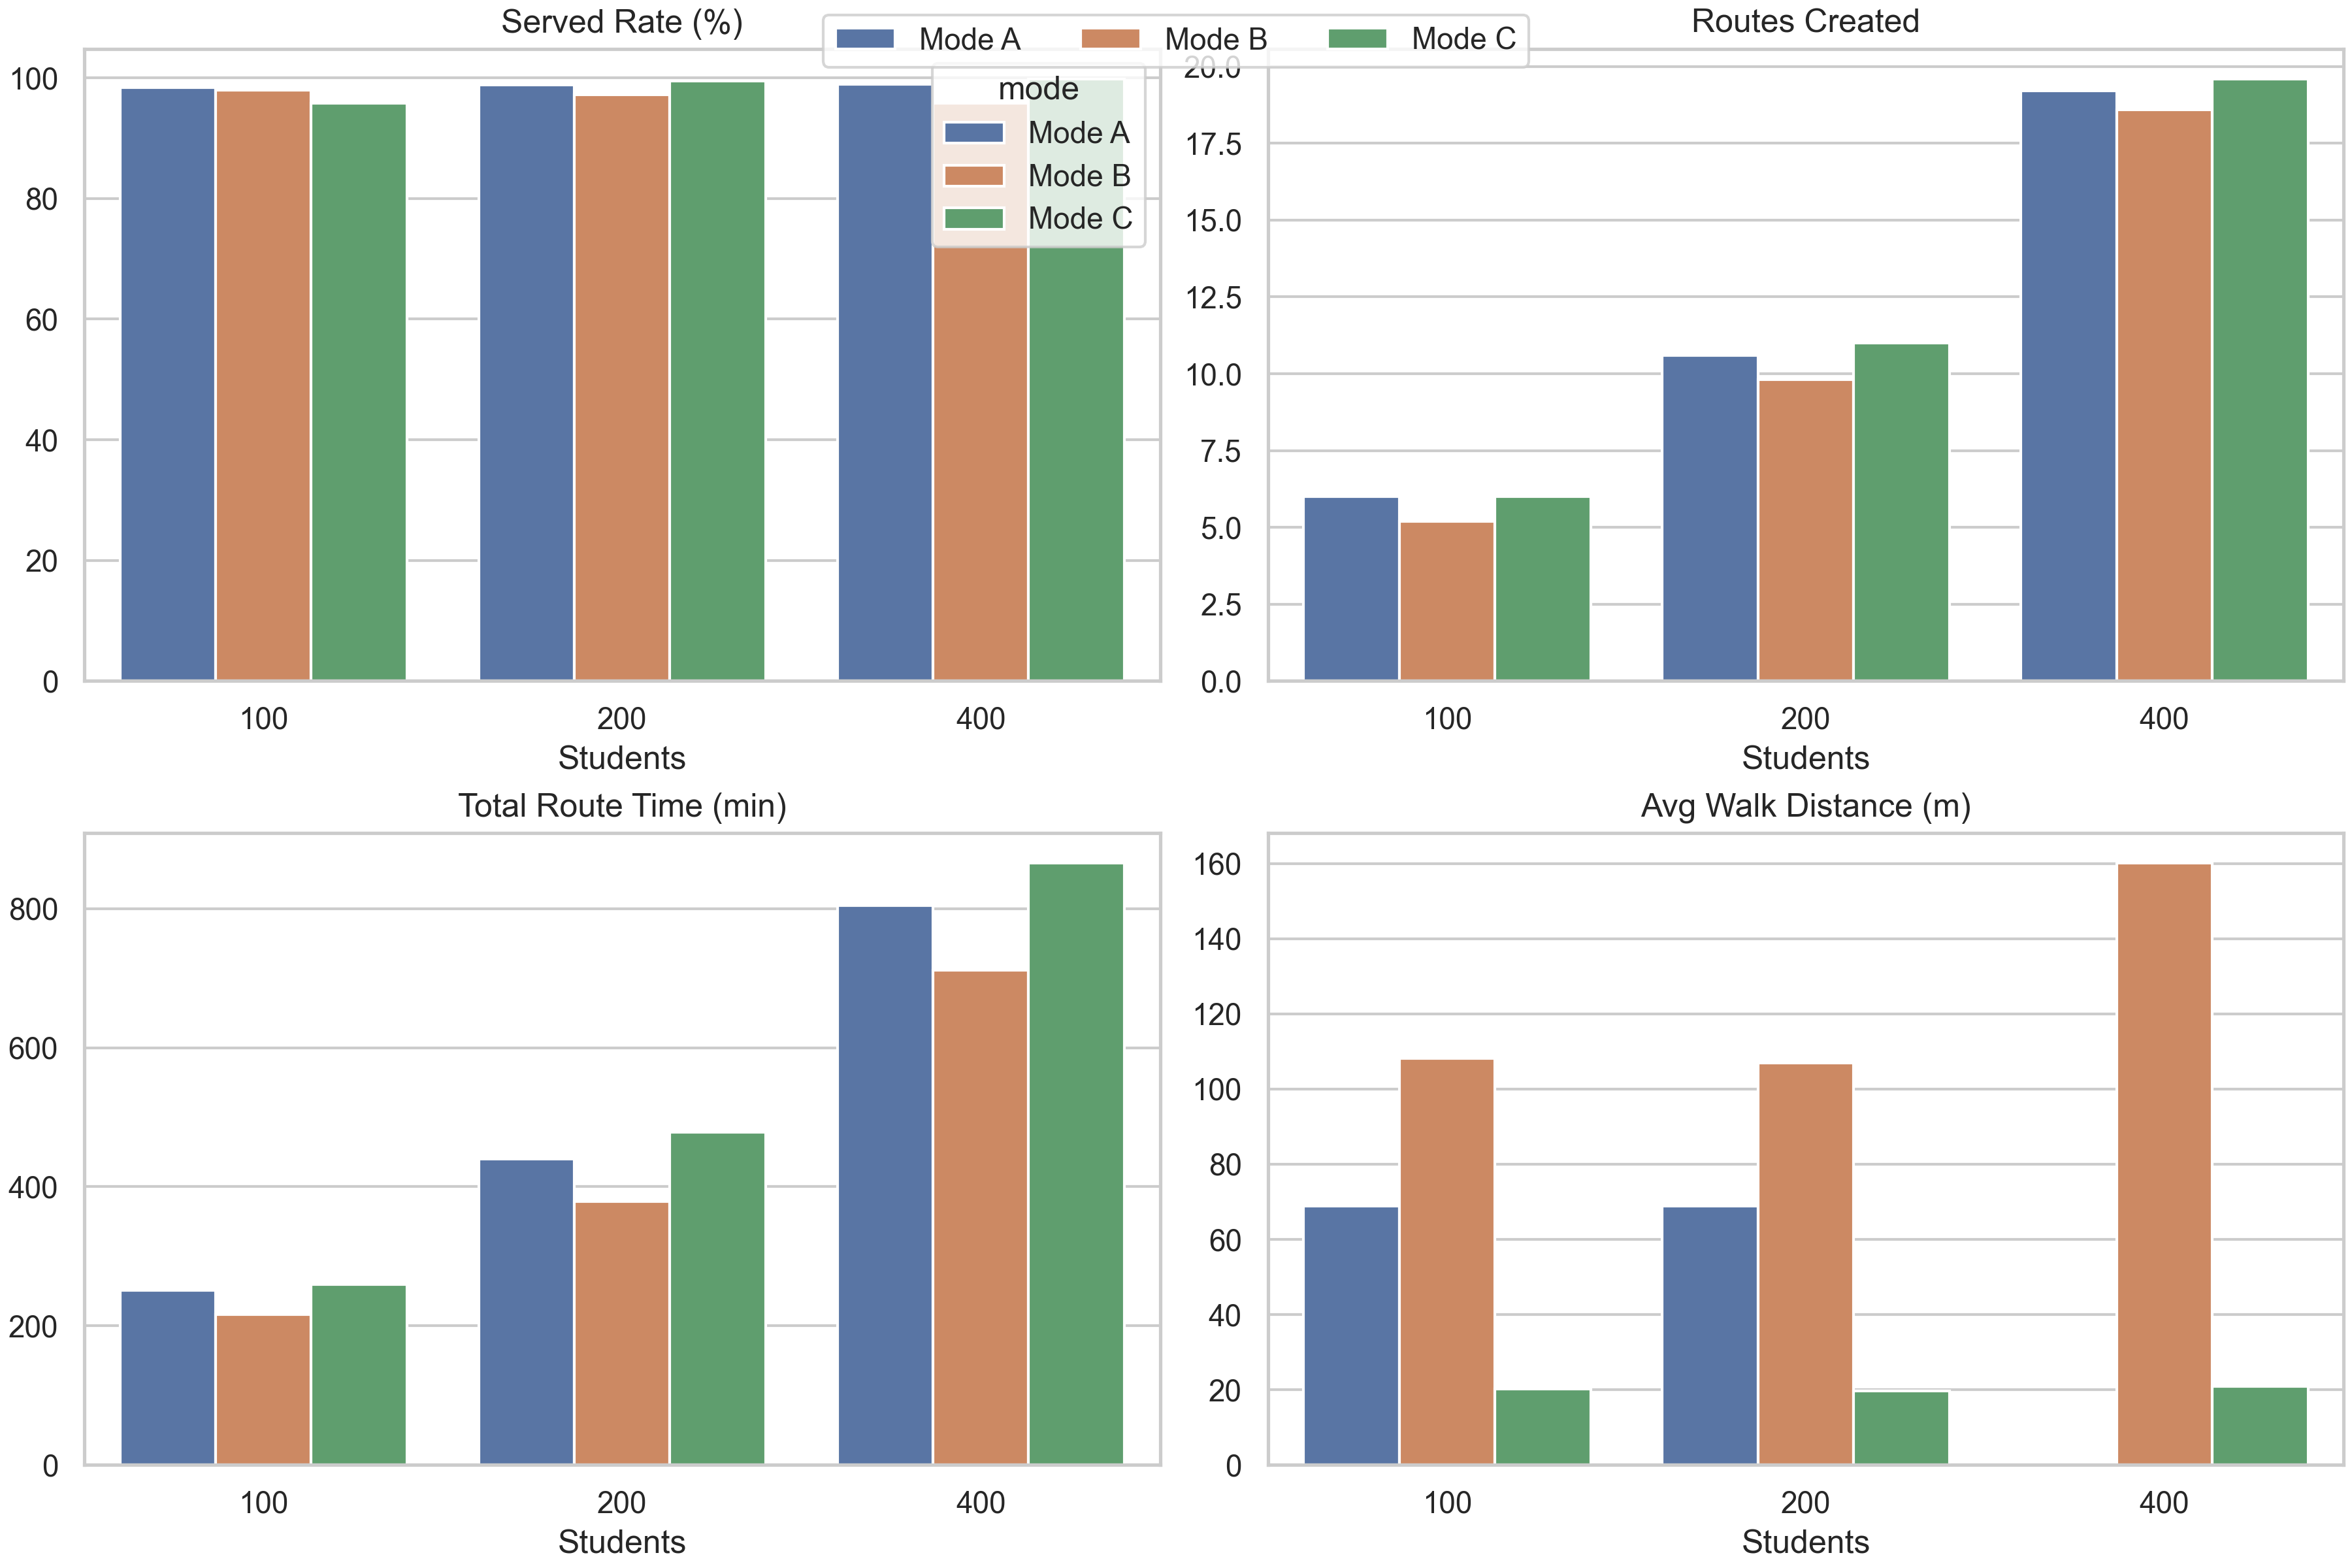
\includegraphics[width=\linewidth]{figures/figure1_mode_comparison.png}
\caption{Mode-level comparison across core outcomes (coverage, routes, route-time, and walking burden) by cohort.}
\label{fig:mode_comparison}
\end{figure}

\begin{figure}[!t]
\centering
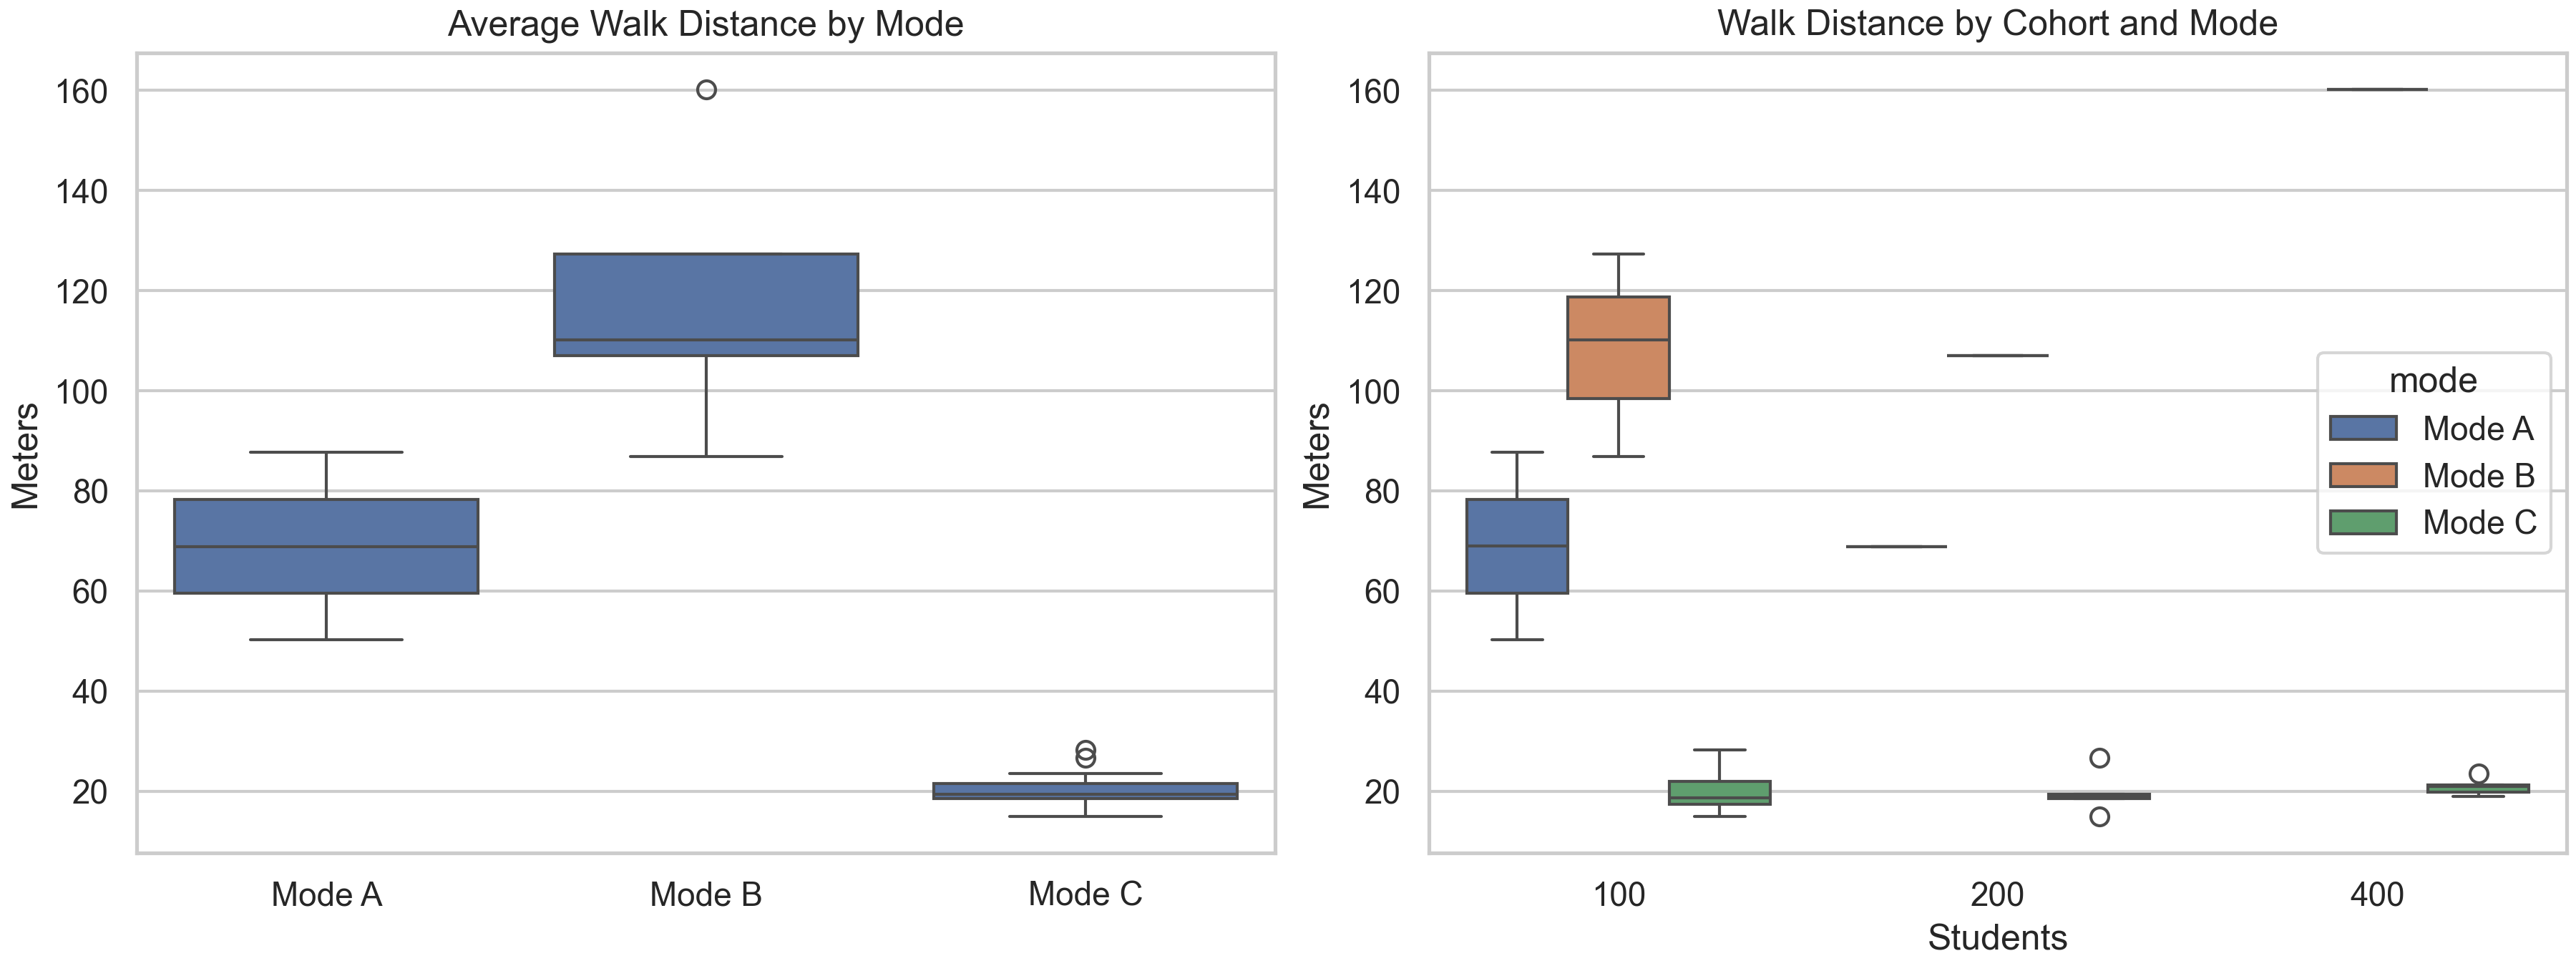
\includegraphics[width=\linewidth]{figures/figure4_walking_distribution.png}
\caption{Walking-distance distributions by mode and cohort.}
\label{fig:walking_distribution}
\end{figure}

\subsubsection{Performance and Scalability}
Runtime and convergence diagnostics indicate scaling pressure as instance size
increases, especially from $|S|=400$ onward. Convergence trajectories
(Figure~\ref{fig:convergence}) show slower improvement blocks and earlier
stagnation under larger candidate spaces, while scalability trends
(Figure~\ref{fig:scalability}) show widening runtime variance at higher $|S|$.

\begin{figure}[!t]
\centering
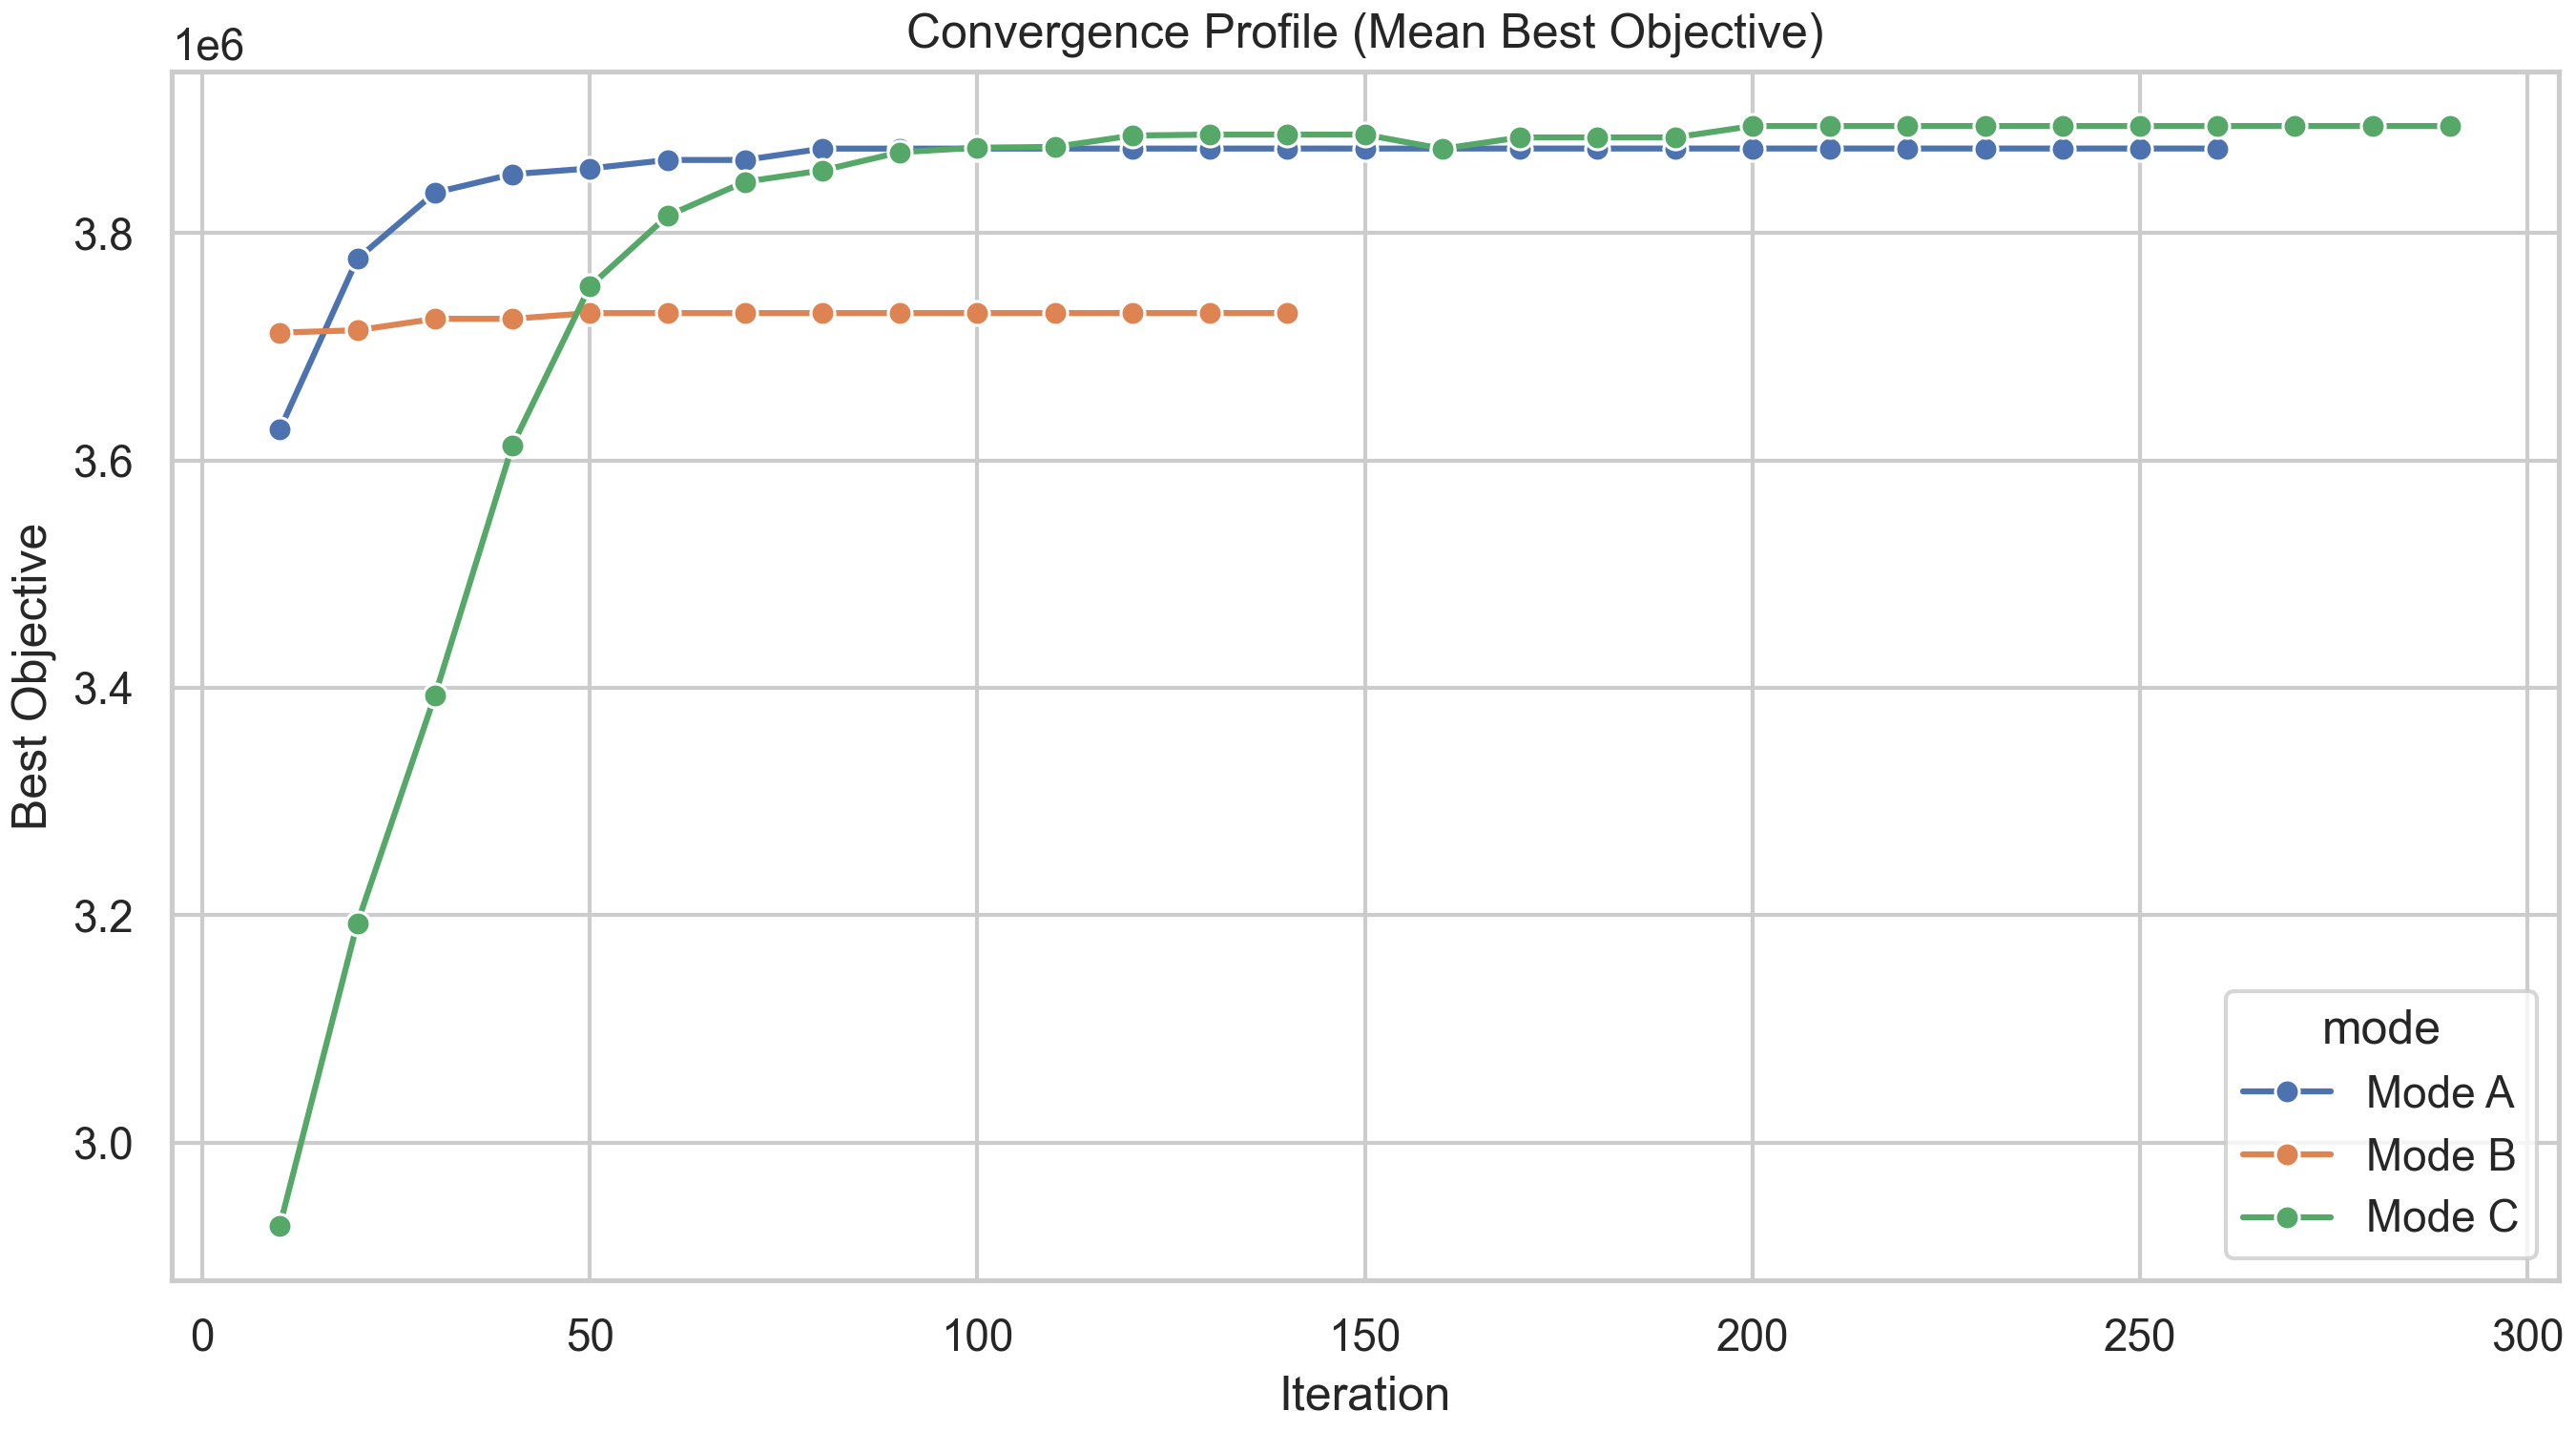
\includegraphics[width=\linewidth]{figures/figure2_convergence_curves.png}
\caption{Mean best-objective convergence profile (shown on representative larger-cohort logs).}
\label{fig:convergence}
\end{figure}

\begin{figure}[!t]
\centering
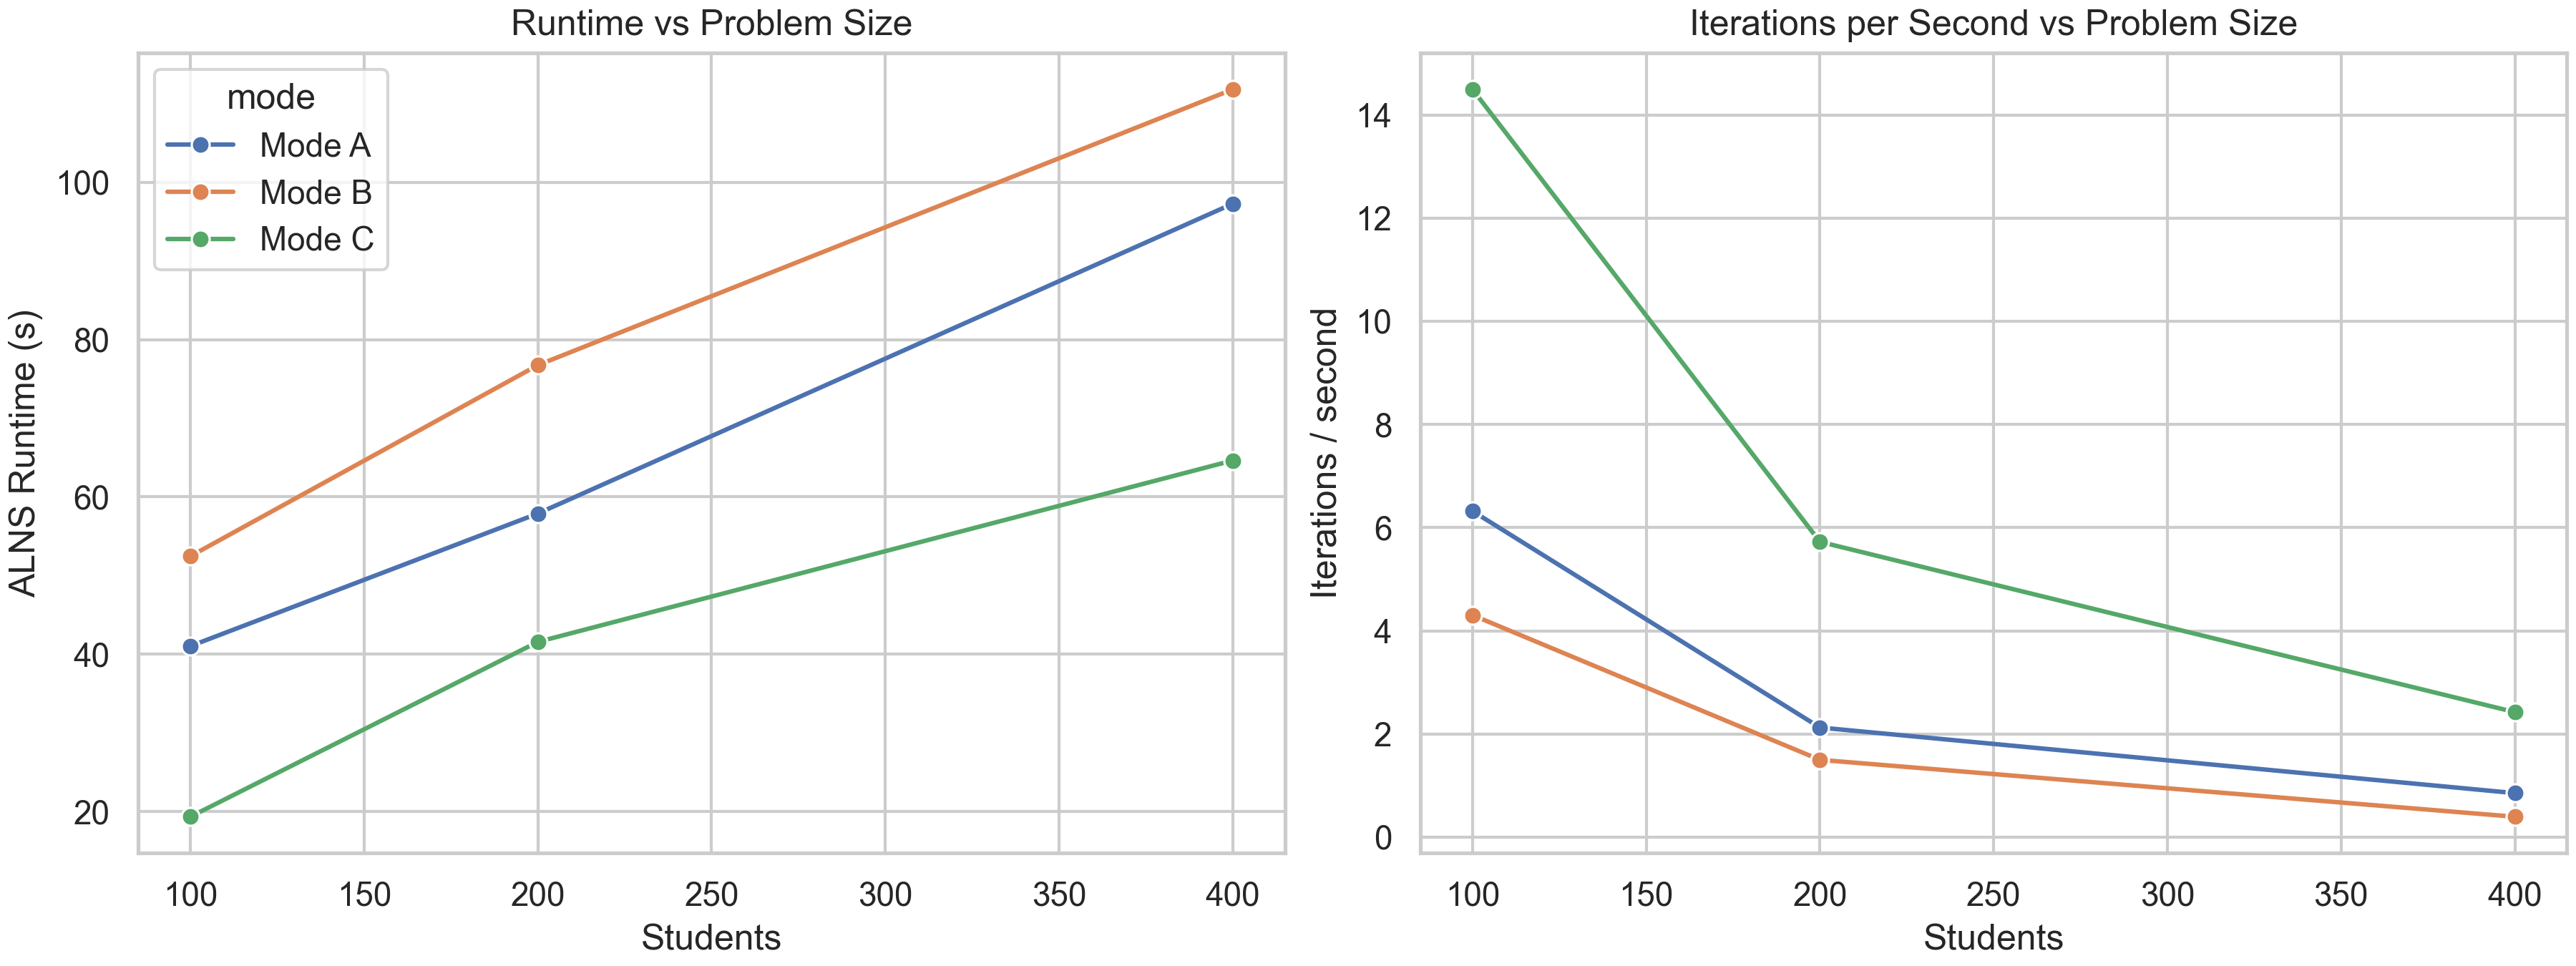
\includegraphics[width=\linewidth]{figures/figure3_scalability_trends.png}
\caption{Scalability trends for runtime and throughput (iterations/second) by mode.}
\label{fig:scalability}
\end{figure}

\subsubsection{Sensitivity Analysis (Optional)}
Assess how key parameter changes (e.g., candidate cap, ride-time multiplier,
or early-stopping settings) affect solution quality and runtime trade-offs.

\section{CONCLUSION}
The experiments show a consistent practical trade-off among efficiency, safety,
and comfort under matched-seed evaluation on complete cohorts
($|S|\in\{100,200,400\}$). Mode B generally improved operational efficiency
relative to Mode A and Mode C, with lower route-time and route-distance across
cohorts (e.g., at $|S|=400$: $711.22\pm62.31$ min and $315.81\pm42.57$ km for
Mode B versus $804.26\pm29.03$ min and $335.07\pm16.90$ km for Mode A).
Mode C generally delivered the highest coverage and the lowest walking burden,
but often at higher route-time than Mode B, confirming a policy trade-off
between operator efficiency and passenger-side convenience.

Inferentially, Wilcoxon paired tests with Holm correction did not yield
statistically significant differences at the current seed count, despite
strongly directional rank-biserial effect sizes in multiple comparisons.
Accordingly, we treat the evidence as robust directional trends rather than
population-level definitive effects.

Future work should expand matched large-scale cohorts and report hardware-fixed
repetitions to tighten uncertainty bands for inferential claims.

%%%%%%%%%%%%%%%%%%%%%%%%%%%%%%%%%%%%%%%%%%%%%%%%%%%%%%%%%%%%%%%%%%%%%%%%%%%%%%%%
\clearpage
\begin{thebibliography}{99}

\bibitem{c1} J. Park and B.-I. Kim, ``The school bus routing problem: A review,'' \textit{European Journal of Operational Research}, vol. 202, no. 2, pp. 311--319, 2010, doi: \href{https://doi.org/10.1016/j.ejor.2009.05.017}{10.1016/j.ejor.2009.05.017}.

\bibitem{c2} K. Wang, Y. Yang, M. Liao, and A. Chen, ``The school bus routing problem: A comprehensive review,'' \textit{European Transport Studies}, vol. 2, Art. no. 100043, 2025, doi: \href{https://doi.org/10.1016/j.ets.2025.100043}{10.1016/j.ets.2025.100043}.

\bibitem{c3} P. Schittekat, J. Kinable, K. Sörensen, M. Sevaux, F. Spieksma, and J. Springael, ``A metaheuristic for the school bus routing problem with bus stop selection,'' \textit{European Journal of Operational Research}, vol. 229, no. 2, pp. 518--528, 2013, doi: \href{https://doi.org/10.1016/j.ejor.2013.02.025}{10.1016/j.ejor.2013.02.025}.

\bibitem{c4} H. I. Calvete, C. Galé, J. A. Iranzo, and P. Toth, ``A partial allocation local search matheuristic for solving the school bus routing problem with bus stop selection,'' \textit{Mathematics}, vol. 8, no. 8, Art. no. 1214, 2020, doi: \href{https://doi.org/10.3390/math8081214}{10.3390/math8081214}.

\bibitem{c5} W. A. Ellegood, S. Solomon, J. North, and J. F. Campbell, ``School bus routing problem: Contemporary trends and research directions,'' \textit{Omega}, vol. 95, Art. no. 102056, 2020, doi: \href{https://doi.org/10.1016/j.omega.2019.03.014}{10.1016/j.omega.2019.03.014}.

\bibitem{c6} F. M. S. Lima, D. S. Pereira, S. V. Conceição, and N. T. R. Nunes, ``A mixed load capacitated rural school bus routing problem with heterogeneous fleet: Algorithms for the Brazilian context,'' \textit{Expert Systems with Applications}, vol. 56, pp. 320--334, 2016, doi: \href{https://doi.org/10.1016/j.eswa.2016.03.005}{10.1016/j.eswa.2016.03.005}.

\bibitem{c7} S. Ropke and D. Pisinger, ``An adaptive large neighborhood search heuristic for the pickup and delivery problem with time windows,'' \textit{Transportation Science}, vol. 40, no. 4, pp. 455--472, 2006, doi: \href{https://doi.org/10.1287/trsc.1050.0135}{10.1287/trsc.1050.0135}.

\end{thebibliography}

\end{document}